\documentclass[11pt, a4paper]{article}

% === PACKAGES ===
\usepackage[utf8]{inputenc}
\usepackage{amsmath}
\usepackage{graphicx}
\usepackage[margin=1in]{geometry} % Standard margin, guide only specifies A4.
\usepackage{setspace}
\usepackage{caption}
\usepackage{tikz}
\usetikzlibrary{shapes.geometric, arrows.meta, positioning, calc}
\usepackage{float}
\usepackage{booktabs}
\usepackage{kotex}
\usepackage{multirow}

% Page numbers at the bottom center.
\usepackage{fancyhdr}
\pagestyle{fancy}
\fancyhf{} % Clear all header and footer fields
\cfoot{\thepage}
\renewcommand{\headrulewidth}{0pt}
\renewcommand{\footrulewidth}{0pt}

% Double spacing for the main body.
\doublespacing

% Input the TikZ style definitions from your graph.tex file
\tikzset{
    title/.style={font=\Large\bfseries},
    block/.style={rectangle, rounded corners, text width=2.5cm, minimum height=1.5cm, text centered, draw=black, fill=gray!20, font=\small\setstretch{0.9}},
    space/.style={rectangle, rounded corners, minimum width=3.5cm, minimum height=3.5cm, draw=black!80, fill=gray!10, text centered, font=\small\setstretch{0.9}},
    output/.style={diamond, aspect=2, minimum size=1.0cm, text centered, draw=black, fill=gray!20, font=\small\setstretch{0.9}},
    main_arrow/.style={thick, -Triangle, line width=1pt},
    update_arrow/.style={thick, dashed, -Triangle, draw=red!80, rounded corners},
    sarc_emb/.style={circle, fill=red!60, draw=black, minimum size=8pt, inner sep=0pt},
    norm_emb/.style={rectangle, fill=blue!60, draw=black, minimum size=8pt, inner sep=0pt},
    force_arrow/.style={-stealth, dashed}
}

% === DOCUMENT START ===
\begin{document}

% Page numbering for Abstract in lowercase roman.
    \pagenumbering{roman}
    \setcounter{page}{1}

% --- COVER PAGE ---
    \begin{titlepage}
        \centering
        \vspace*{3cm}
        {\huge SimSCLSD: A Simple Framework for Supervised Contrastive Learning of Sarcasm Detection}

        \vspace{1cm}
        {\large 반어 표현 탐지를 위한 단순 지도 대조 학습 프레임워크}
        \vfill

        {\large 2025년 11월}
        \vspace{1.5cm}

        {\large 서울대학교 공과대학} \\
        {\large 전기·정보공학부}

        \vspace{1cm}
        {\large 엄 태 윤}

    \end{titlepage}

% --- APPROVAL PAGE ---
    \begin{titlepage}
        \centering
        \vspace*{2cm}
        {\huge SimSCLSD: A Simple Framework for Supervised Contrastive Learning of Sarcasm Detection}

        \vspace{1cm}
        {\large 반어 표현 탐지를 위한 단순 지도 대조 학습 프레임워크}

        \vfill
        {\large 지도교수 심 규 석}

        \vspace{1cm}
        {\large 이 논문을 공학학사 학위논문으로 제출함}

        \vspace{0.5cm}
        {\large 2025년 11월}

        \vspace{0.5cm}
        {\large 서울대학교 공과대학} \\
        {\large 전기·정보공학부}

        \vspace{0.5cm}
        {\large 엄 태 윤}

        \vspace{1.5cm}
        {\large 엄태윤의 학사 학위논문을 인준함}

        \vspace{0.5cm}
        {\large 2025년 \quad 월 \quad 일}

        \vspace{0.5cm}
        {\large 지도교수 \_\_\_\_\_\_\_\_\_\_ (인)}

    \end{titlepage}

% --- ABSTRACT ---
    \begin{center}
    {\Large\bfseries Abstract}
    \end{center}

    \vspace{1em}

    Detecting sarcasm, especially in online discourses, is a significant challenge in Natural Language Processing (NLP).
    Sarcasm is an intricate form of speech where the actual intent is often the opposite of the literal one and is highly dependent on the surrounding conversational context.
    While pre-trained Transformer-based language models have become standard baselines, they are typically fine-tuned using a Cross-Entropy (CE) loss.
    This approach may not be optimal for learning discriminative representations, especially for a nuanced task like sarcasm where the boundary between classes is subtle.

    In this paper, we propose SimSCLSD, a Simple framework for Supervised Contrastive Learning of Sarcasm Detection, which introduces a two-stage training process.
    First, a RoBERTa-based encoder undergoes a contrastive pre-training phase on the task-specific dataset.
    This stage utilizes a supervised contrastive loss to learn a discriminative embedding space, pulling representations of same-label examples (e.g., two sarcastic comments) together while pushing representations of different-label examples apart.
    Second, the adapted model is fine-tuned using a standard CE loss for the final classification.
    We investigate critical implementation details, such as the use of mean-pooled sequence representations for the contrastive task versus \texttt{[CLS]} token representations for the classification task.

    We evaluate our approach on the two datasets from the FigLang 2020 Sarcasm Detection shared task: Reddit and Twitter.
    Our experiments demonstrate that this contrastive pre-training step can effectively create more separable representations, showing its potential as an effective intermediate step for fine-tuning transformers on nuanced, context-dependent classification tasks.

    \vspace{2em}
    \noindent
    \textbf{keywords:} sarcasm detection, supervised contrastive learning, representation learning, text classification, conversational context, embedding space

    \vspace{1em}
    \noindent
    \textbf{Student Number: 2019-18535}

    \clearpage

% --- TABLE OF CONTENTS ---
    \tableofcontents

    \clearpage

% --- MAIN BODY ---
    \pagenumbering{arabic}
    \setcounter{page}{1}

    \section{Related Work}
    Our research is positioned at the intersection of three key areas: sarcasm detection as a context-dependent task, the use of Transformer-based models for this task, and the application of supervised contrastive learning to improve representation quality in NLP\@.

    \subsection{Sarcasm Detection and Context}
    Sarcasm detection is typically framed as a binary classification task (sarcastic vs. non-sarcastic).
    It is a critical sub-problem in NLP, as accurately identifying sarcastic intent is essential for understanding a user's true sentiments and beliefs.
    The primary challenge is that sarcastic utterances often use positive words to convey a negative meaning, making the literal text misleading.

    Researchers have shown that for both humans and computers, conversational context is vital for correctly identifying sarcasm.
    An isolated response may be ambiguous, but its sarcastic nature becomes clear when paired with the preceding conversation~\cite{ghosh2020report}.
    The FigLang 2020 shared task, the source of our datasets, was specifically designed to benchmark models on their ability to leverage this conversational context~\cite{ghosh2020report}.

    \subsection{Transformer Models for Sarcasm Detection}
    The FigLang 2020 shared task demonstrated that pre-trained Transformer models (PLRMs) are the dominant architecture for this problem~\cite{ghosh2020report}.
    Top-performing teams almost universally adopted variants of BERT~\cite{devlin2019bert} and RoBERTa~\cite{liu2019roberta, dong2020transformer, jaiswal2020neural}.
    The primary architectural challenge then became how to best incorporate the conversational context.

    Several strategies emerged from the shared task:
    \begin{itemize}
        \item \textbf{Concatenation:} The most common approach was to concatenate the context and the target response into a single input sequence, which is then fed into the Transformer~\cite{dong2020transformer}.
        Dong et al. (2020) showed this context-aware model significantly outperformed a target-oriented model that only used the response~\cite{dong2020transformer}.

        \item \textbf{Input Formatting:} Pant and Dadu (2020)~\cite{pant2020sarcasm} demonstrated that the *method* of concatenation matters.
        They found that fine-tuning RoBERTa with a special separator token between the context and the response yielded a performance improvement on the Reddit dataset compared to simple concatenation~\cite{pant2020sarcasm}.
        Our work adopts this separator-based format.

        \item \textbf{Context Length and Ensembling:} A key finding from several top teams was that using the entire context history was not always optimal.
        Jaiswal (2020)~\cite{jaiswal2020neural} and Lee et al. (2020)~\cite{lee2020augmenting} both found that using only the most recent three context turns provided the best performance, suggesting that older context may add noise~\cite{jaiswal2020neural, lee2020augmenting}.
        Both teams also employed an ensembling strategy, combining models trained on different context lengths~\cite{jaiswal2020neural, lee2020augmenting}.

        \item \textbf{Novel Formulations:} Other approaches included hierarchical models~\cite{srivastava2020novel} and adapting Aspect-Based Sentiment Analysis (ABSA) models, which treat the context as the aspect and the response as the target~\cite{ataei2020applying}.
        The winning team, Lee et al. (2020)~\cite{lee2020augmenting}, attributed their success to a novel data augmentation technique (CRA) and a complex pooling mechanism (NeXtVLAD).
    \end{itemize}
    While these approaches focused on architectural changes, input formatting, and data augmentation, our work investigates a complementary approach: optimizing the learning objective itself.

    \subsection{Supervised Contrastive Learning for NLP}
    The vast majority of Transformer-based classifiers are fine-tuned using a standard Cross-Entropy (CE) loss.
    However, CE has known limitations; it optimizes for correct classification but does not explicitly enforce a discriminative embedding space.
    This can lead to poor margins and instability, especially on noisy or nuanced datasets.

    Contrastive Learning has emerged as a powerful alternative for representation learning.
    It was popularized in self-supervised vision (e.g., SimCLR~\cite{chen2020simple}), where the goal is to pull representations of augmented views of the same image (positives) together while pushing representations of all other images (negatives) apart.

    Our work uses Supervised Contrastive (SupCon) Learning, an extension formalized by Khosla et al. (2020)~\cite{khosla2020supervised} that leverages label information.
    Instead of only pulling augmented views of one sample together, the SupCon loss aims to pull all samples belonging to the same class into a tight cluster in the embedding space, while simultaneously pushing apart clusters of samples from different classes.

    This technique has been successfully applied as an intermediate training step for large language models.
    Moukafih et al. (2022)~\cite{moukafih2022simscl} proposed SimSCL, a simple supervised contrastive framework for text representation, showing its effectiveness on sentiment classification.
    Li et al. (2021)~\cite{li2021simclad} also proposed a similar continual contrastive pre-training to adapt a general-purpose model (like BERT) to a specific task's feature distribution.
    Our work builds on these ideas, extending the SimSCL methodology to the more complex, context-dependent task of sarcasm detection.

    \section{Proposed Method}
    Our approach, SimSCLSD, is a two-stage training framework designed to improve the performance of Transformer models on context-aware sarcasm detection.
    The core idea is to conceptually separate the task of learning discriminative feature representations from the task of learning a classification boundary.
    First, we adapt a pre-trained RoBERTa encoder using a Supervised Contrastive (SupCon) objective.
    Second, we fine-tune a simple classifier head on top of this adapted encoder using a standard Cross-Entropy (CE) objective.

    \subsection{Model Architecture and Input Format}
    Our model consists of a RoBERTa-base encoder~\cite{liu2019roberta} followed by a single linear layer that serves as the classifier.
    A key distinction in our architecture is the use of two different pooling strategies, one for each training stage, to best suit the objective of that stage.

    \begin{itemize}
        \item For contrastive pre-training (Stage 1), we use a mean-pooling operation over the final hidden states of all tokens.
        This produces a single vector $z$ that represents the entire input sequence, a method well-suited for representation learning.
        \item For classification fine-tuning (Stage 2), we use the standard \texttt{[CLS]} token embedding as the input to the linear classifier, as this representation is specifically optimized during pre-training for classification tasks~\cite{devlin2019bert}.
    \end{itemize}

    Following the findings of Pant and Dadu (2020)~\cite{pant2020sarcasm}, we format all inputs by concatenating the conversational context and the target response.
    All preceding context turns are joined by a special separator token, \texttt{[SEP]}, and another \texttt{[SEP]} token is used to separate the full context from the target response.
    This creates a single input sequence formatted as:
    \begin{center}
        \texttt{[CLS] context\_1 [SEP] ... [SEP] target\_response [EOS]}
    \end{center}

    \subsection{Two-Stage Training Framework}
    The model architecture is trained using a two-stage process, which is illustrated in Figures ~\ref{fig:stage1} and Figure~\ref{fig:stage2}.

    \subsubsection{Stage 1: Supervised Contrastive Pre-training}
    As illustrated in Figure~\ref{fig:stage1}, the first stage trains the encoder to produce separable feature representations.
    The mean-pooled representation $z$ is optimized using a Supervised Contrastive Loss ($\mathcal{L}_{\text{SupCon}}$).
    This loss, based on the $\mathcal{L}_{\text{out}}^{\sup}$ formulation from Khosla et al. (2020)~\cite{khosla2020supervised}, is defined for a batch of $N$ samples as:

    \[
        \mathcal{L}_{\text{SupCon}} = \sum_{i \in I} \frac{-1}{|P(i)|} \sum_{p \in P(i)} \log \frac{\exp(z_i \cdot z_p / \tau)}{\sum_{a \in A(i)} \exp(z_i \cdot z_a / \tau)}
    \]

    Where $i$ is an anchor sample, $z_i$ is its normalized embedding, $P(i)$ is the set of positive samples in the batch, $A(i)$ is the set of all other samples, and $\tau$ is temperature.
    This objective function explicitly trains the encoder to maximize the similarity between samples from the same class(attract) while minimizing the similarity between samples from different classes(repel).

    \begin{figure}[H]
        \centering
        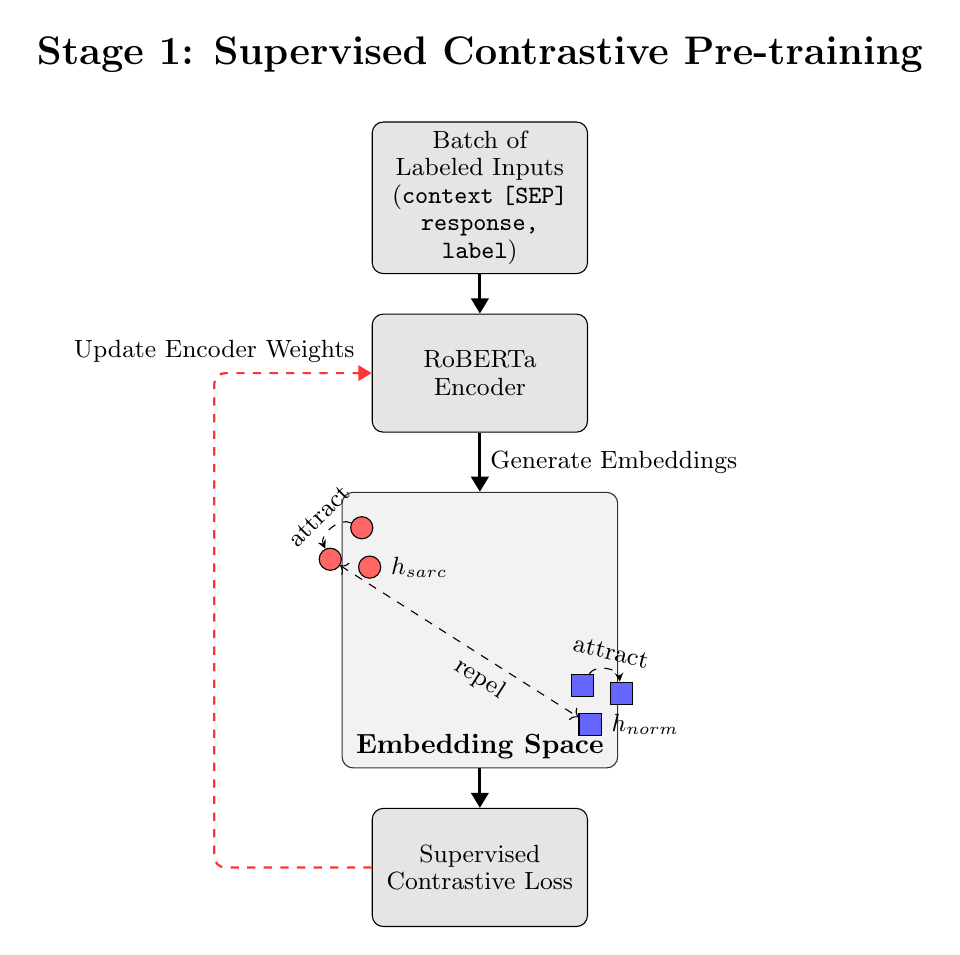
\begin{tikzpicture}[node distance=.5cm]

    % --- Title ---
    \node (title) [title] {Stage 1: Supervised Contrastive Pre-training};

    % --- Input Data ---
    \node (input) [block, below=of title] {Batch of Labeled Inputs \\ \small(\texttt{context [SEP] response, label})};

    % --- RoBERTa Encoder ---
    \node (encoder) [block, below=of input] {RoBERTa Encoder};
    \draw [main_arrow] (input) -- (encoder);

    % --- Embedding Space ---
    \node (emb_space) [space, below=.75cm of encoder] {};
    \node [above] at (emb_space.south) {\textbf{Embedding Space}};
    \draw [main_arrow] (encoder) -- (emb_space) node [midway, right, font=\small] {Generate Embeddings};

    % Coordinates for embedding clusters
    \coordinate (c1) at ($(emb_space.center)+(-1.5, 1.3)$); % Sarcastic cluster
    \coordinate (c2) at ($(emb_space.center)+(1.3, -0.7)$); % Not Sarcastic cluster

    % Sarcastic Embeddings (Circles)
    \node[sarc_emb] (s1) at (c1) {};
    \node[sarc_emb] (s2) at ($(c1)+(-0.4,-0.4)$) {};
    \node[sarc_emb, label={[font=\small]right:$h_{sarc}$}] (s3) at ($(c1)+(0.1,-0.5)$) {};

    % Not Sarcastic Embeddings (Squares)
    \node[norm_emb] (n1) at (c2) {};
    \node[norm_emb] (n2) at ($(c2)+(0.5,-0.1)$) {};
    \node[norm_emb, label={[font=\small]right:$h_{norm}$}] (n3) at ($(c2)+(0.1,-0.5)$) {};

    % Force arrows illustrating the contrastive objective
    \draw[force_arrow, black, bend right=70] (s1) to node[midway, above, sloped, font=\small] {attract} (s2);
    \draw[force_arrow, black, bend left=70] (n1) to node[midway, above, sloped, font=\small] {attract} (n2);
    \draw[force_arrow, black, <->] (s2) to node[midway, below right, sloped, font=\small] {repel} (n3);

    % --- Loss Function ---
    \node (loss) [block, below=of emb_space] {Supervised Contrastive Loss};
    \draw [main_arrow] (emb_space) -- (loss);

    % --- Weight Update Path ---
    \draw [update_arrow] (loss.west) -- ++(-2,0) |- (encoder.west)
    node [midway, above, font=\small] {Update Encoder Weights};

\end{tikzpicture}
        \caption{Stage 1: Supervised Contrastive Pre-training. The encoder learns to map same-label inputs into nearby clusters and different-label inputs into distant clusters using a mean-pooled representation.}
        \label{fig:stage1}
    \end{figure}

    \subsubsection{Stage 2: Classification Fine-tuning}
    As shown in Figure~\ref{fig:stage2}, the second stage trains the classifier.
    The encoder weights are loaded from Stage 1, and a new linear classification head is added.
    or this stage, we use the standard \texttt{[CLS]} token embedding as the input to the classifier.

    This classifier is then trained using a standard Cross-Entropy (CE) Loss.
    A key feature of this stage is the use of differential learning rates.
    The pre-trained encoder is fine-tuned with a low learning rate, while the new classification head is trained with a higher learning rate.
    This strategy allows the classifier to adapt to the new feature space without causing catastrophic forgetting in the underlying encoder.

    \begin{figure}[H]
        \centering
        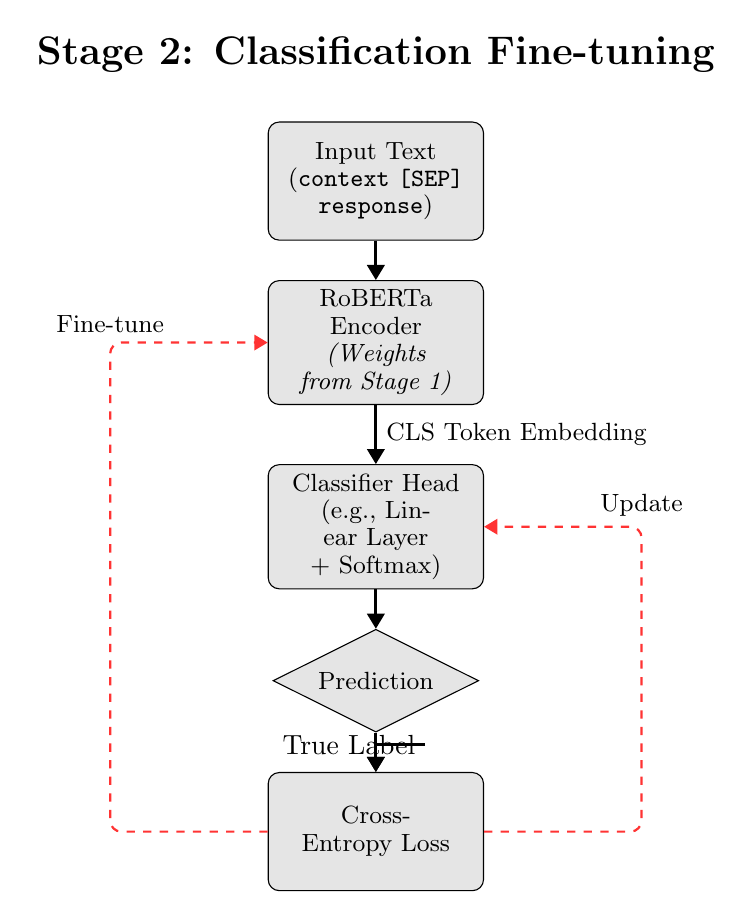
\begin{tikzpicture}[node distance=.5cm]

    % --- Title ---
    \node (title) [font=\Large\bfseries] {Stage 2: Classification Fine-tuning};

    % --- Input Data ---
    \node (input) [block, below=of title] {Input Text \\ \small(\texttt{context [SEP] response})};

    % --- RoBERTa Encoder ---
    \node (encoder) [block, below=of input] {RoBERTa Encoder \\ \small\textit{(Weights from Stage 1)}};
    \draw [main_arrow] (input) -- (encoder);

    % --- Classifier Head ---
    \node (classifier) [block, below=.75cm of encoder] {Classifier Head \\ \small(e.g., Linear Layer + Softmax)};
    \draw [main_arrow] (encoder) -- (classifier) node [midway, right, font=\small] {CLS Token Embedding};

    % --- Final Prediction ---
    \node (prediction) [output, below=of classifier] {Prediction};
    \draw [main_arrow] (classifier) -- (prediction);

    % --- Loss Calculation (Revised Style) ---
    \node (loss) [block, below=of prediction] {Cross-Entropy Loss};
    \draw [main_arrow] (prediction) -- (loss);

    % Replace the block with a simple text node for the label
    \node (label_text) [above left=0.1cm and -2cm of loss] {True Label};
    \draw [main_arrow] (label_text) -| (loss.north);

    % --- Weight Update Paths ---
    % Path to update the classifier (rerouted to the right)
    \draw [update_arrow] (loss.east) -- ++(2,0) |- (classifier.east)
    node [midway, above, font=\small] {Update};

    % Path to update the main encoder (originating from a clean point)
    \draw [update_arrow] (loss.west) -- ++(-2,0) |- (encoder.west)
    node [midway, above, font=\small] {Fine-tune};

\end{tikzpicture}
        \caption{Stage 2: Classification Fine-tuning. The adapted encoder from Stage 1 is used as a base, and a new classifier head is trained using the \texttt{[CLS]} token representation and a Cross-Entropy loss.}
        \label{fig:stage2}
    \end{figure}

    \section{Experiments}

    \subsection{Datasets}
    We evaluate our framework on the two datasets provided by the FigLang 2020 Shared Task on Sarcasm Detection~\cite{ghosh2020report}.
    Both datasets are framed as a binary classification task (sarcastic vs. non-sarcastic) and include conversational context.
    \begin{itemize}
        \item \textbf{FigLang-Reddit:} A dataset of 4,400 training samples and 1,800 test samples from Reddit.
        Sarcastic posts are self-annotated by users with an \texttt{/s} marker.
        \item \textbf{FigLang-Twitter:} A dataset of 5,000 training samples and 1,800 test samples from Twitter.
        Sarcastic tweets were collected using hashtags like \#sarcasm and \#sarcastic.
    \end{itemize}
    For all experiments, we use a 90/10 split of the provided training data to create our own training and validation sets, respectively.

    \subsection{Experimental Setup}
    We compare two models to evaluate the effectiveness of our proposed framework.
    All models use RoBERTa-base~\cite{liu2019roberta} as the encoder and a batch size of 64.
    All training runs use early stopping on the fine-tuning stage with a patience of 2, based on the validation macro F1-score.

    \textbf{Baseline (Ablation):} This is a standard fine-tuning approach.
    The model is trained for up to 10 epochs using only the Cross-Entropy loss.
    For the Twitter dataset, a learning rate of $3 \times 10^{-5}$ was used for the classifier and $5 \times 10^{-7}$ for the encoder.
    For the Reddit dataset, learning rates of $3 \times 10^{-5}$ and $1 \times 10^{-6}$ were used, respectively.
    This represents the ablation model, as it omits our Stage 1 pre-training.

    \textbf{SimSCLSD (Ours):} This is our proposed two-stage framework.
    \begin{itemize}
        \item Stage 1 (Contrastive): The encoder is trained for 20 epochs using our Supervised Contrastive Loss with a learning rate of $5 \times 10^{-5}$ and a temperature $\tau$ of $0.2$.
        The learning rate is $3 \times 10^{-5}$ for the entire model.
        Supervised Contrastive Loss with a learning rate of $5 \times 10^{-5}$ and a temperature $\tau$ of $0.2$.
        \item Stage 2 (Fine-tuning): The adapted encoder is fine-tuned for up to 10 epochs using a Cross-Entropy loss.
        For the Twitter dataset, learning rates were $3 \times 10^{-5}$ (classifier) and $5 \times 10^{-7}$ (encoder).
        For the Reddit dataset, they were $1 \times 10^{-5}$ (classifier) and $1 \times 10^{-6}$ (encoder).
    \end{itemize}
    The dropout rate was set to 0.1 for Twitter and 0.5 for the Reddit SimSCLSD model.

    \subsection{Classification Results}
    We evaluate all models on the official test set using Macro Precision, Recall, and F1-score.
    The model checkpoint that performed best on the validation set was used for final testing.
    The results of our experiments are presented in Table~\ref{tab:results}.

    \begin{table}[H]
        \centering
        \caption{Comparison of dev and test set performance between the Baseline (standard fine-tuning) and our proposed SimSCLSD framework. All metrics are Macro-averaged.}
        \label{tab:results}
        \begin{tabular}{l c c c c c}
            \toprule
            \textbf{Model} & \textbf{Dataset} & \textbf{Split} & \textbf{Precision} & \textbf{Recall} & \textbf{Macro F1} \\
            \midrule
            \multirow{2}{*}{Baseline (Ablation)} & \multirow{2}{*}{Reddit} & Dev & 0.5679 & 0.5568 & 0.5379 \\
            & & Test & 0.5244 & 0.5228 & 0.5148 \\
            \midrule
            \multirow{2}{*}{\textbf{SimSCLSD (Ours)}} & \multirow{2}{*}{\textbf{Reddit}} & Dev & 0.6974 & 0.6955 & 0.6947 \\
            & & \textbf{Test} & \textbf{0.6166} & \textbf{0.6139} & \textbf{0.6116} \\
            \midrule
            \multirow{2}{*}{Baseline (Ablation)} & \multirow{2}{*}{Twitter} & Dev & 0.7352 & 0.7300 & 0.7285 \\
            & & Test & 0.7047 & 0.6861 & 0.6788 \\
            \midrule
            \multirow{2}{*}{\textbf{SimSCLSD (Ours)}} & \multirow{2}{*}{\textbf{Twitter}} & Dev & 0.8486 & 0.8480 & 0.8479 \\
            & & \textbf{Test} & \textbf{0.7477} & \textbf{0.7461} & \textbf{0.7457} \\
            \bottomrule
        \end{tabular}
    \end{table}

    The results, presented in Table~\ref{tab:results}, clearly demonstrate the benefit of our two-stage approach.
    On the FigLang-Reddit test dataset, our SimSCLSD framework achieves a Macro F1-score of 0.6116, a significant improvement of 9.68 percentage points compared to the 0.5148 F1-score of the baseline model.
    This trend is also visible on the FigLang-Twitter dataset, where our model (0.7457 F1) outperforms the baseline (0.6788 F1) by 6.69 percentage points.
    These results suggest that by first training the encoder to explicitly separate the classes in the embedding space (Stage 1), we provide a much better initialization for the final classifier (Stage 2), leading to superior performance.

    \section{Conclusion}
    In this paper, we proposed and evaluated SimSCLSD, a simple two-stage framework for context-aware sarcasm detection.
    We demonstrated that preceding a standard classification fine-tuning stage with a task-specific supervised contrastive pre-training stage is an effective method for improving performance.

    Our model was evaluated on the two datasets from the FigLang 2020 shared task~\cite{ghosh2020report}, Reddit and Twitter.
    The experimental results show that our SimSCLSD framework substantially outperforms a strong baseline, achieving an absolute Macro F1-score improvement of 9.7\%p on the Reddit dataset and 6.7\%p on the Twitter dataset.
    This confirms our central hypothesis: for complex, context-dependent nuanced tasks like sarcasm detection, explicitly training the encoder to produce a more discriminative and well-separated embedding space provides a superior foundation for the final classifier.

    This study was limited to the RoBERTa-base model.
    Future work could explore the impact of this framework on larger language models.
    Furthermore, the promising results suggest this two-stage contrastive pre-training approach could be a valuable and generalizable method for other complex NLP classification tasks that depend on subtle contextual cues, such as irony, humor, or stance detection.

% --- REFERENCES ---
    \bibliographystyle{IEEEtran}
    \bibliography{references}

\end{document}



